\documentclass{article}
\usepackage[utf8]{inputenc}
\usepackage{authblk}
\usepackage{setspace}
\usepackage[margin=1.25in]{geometry}
\usepackage{graphicx}
\graphicspath{ {./figures/} }
\usepackage{amsmath,amssymb,amsfonts}
\usepackage{booktabs}
\usepackage{natbib}
\usepackage{hyperref}
\hypersetup{colorlinks=true, linkcolor=blue, citecolor=blue, urlcolor=blue}

\title{\textbf{Proximal Policy Optimisation for Multi-Asset ETF Allocation under Transaction Costs}}
\author[1]{hypoq autonomous research harness}
\affil[1]{Hypothesis $\times$ Quant}
\date{\today}
\onehalfspacing

\begin{document}
\maketitle

\begin{abstract}
\noindent \textbf{Hypothesis:} $H_0$: the Sharpe ratio of a PPO allocation policy does not exceed that of daily-rebalanced equal weight; $H_1$: it does \\
\textbf{Data:} Total returns of SPY, TLT, GLD, EEM, HYG; training before 2023, out-of-sample 2023-02-01 to 2026-10-22 (935 days) \\
\textbf{Method:} PPO (3 seeds, 120,000 steps each, averaged), softmax weights, 5 bps cost per unit turnover, decision at close $t$ applied to day $t{+}1$, one-sided stationary-bootstrap test of the Sharpe difference \\
\textbf{Results:} PPO Sharpe 0.18 vs equal weight 1.17 (difference -0.99, $p=1.000$). Decision: \textbf{REJECTED}
\end{abstract}

\section{Design}
The environment exposes the last 20 daily returns of each asset (scaled by training volatility) and the current drifted weights. The agent outputs unconstrained scores mapped to long-only fully invested weights by a softmax; reward is the log net return. Training episodes are random one-year windows before 2023; the test period is simulated once and never used for tuning \citep{moody2001learning}.

\section{Results}
\begin{table}[h!]
\centering
\caption{Out-of-sample performance net of 5 bps cost per unit turnover}
\begin{tabular}{lcccc}
\toprule
Strategy & Ann. return & Ann. vol. & Sharpe & Max drawdown \\
\midrule
PPO ensemble & 1.34\% & 11.16\% & 0.18 & -15.1\% \\
Equal weight & 12.05\% & 10.19\% & 1.17 & -8.7\% \\
SPY buy-and-hold & 20.06\% & 14.82\% & 1.31 & -18.8\% \\
60/40 SPY/TLT & 10.60\% & 11.08\% & 0.96 & -12.7\% \\
\bottomrule
\end{tabular}
\end{table}


The ensemble policy turns over 64.4\% of the portfolio per day on average.

\begin{figure}[h!]
\centering
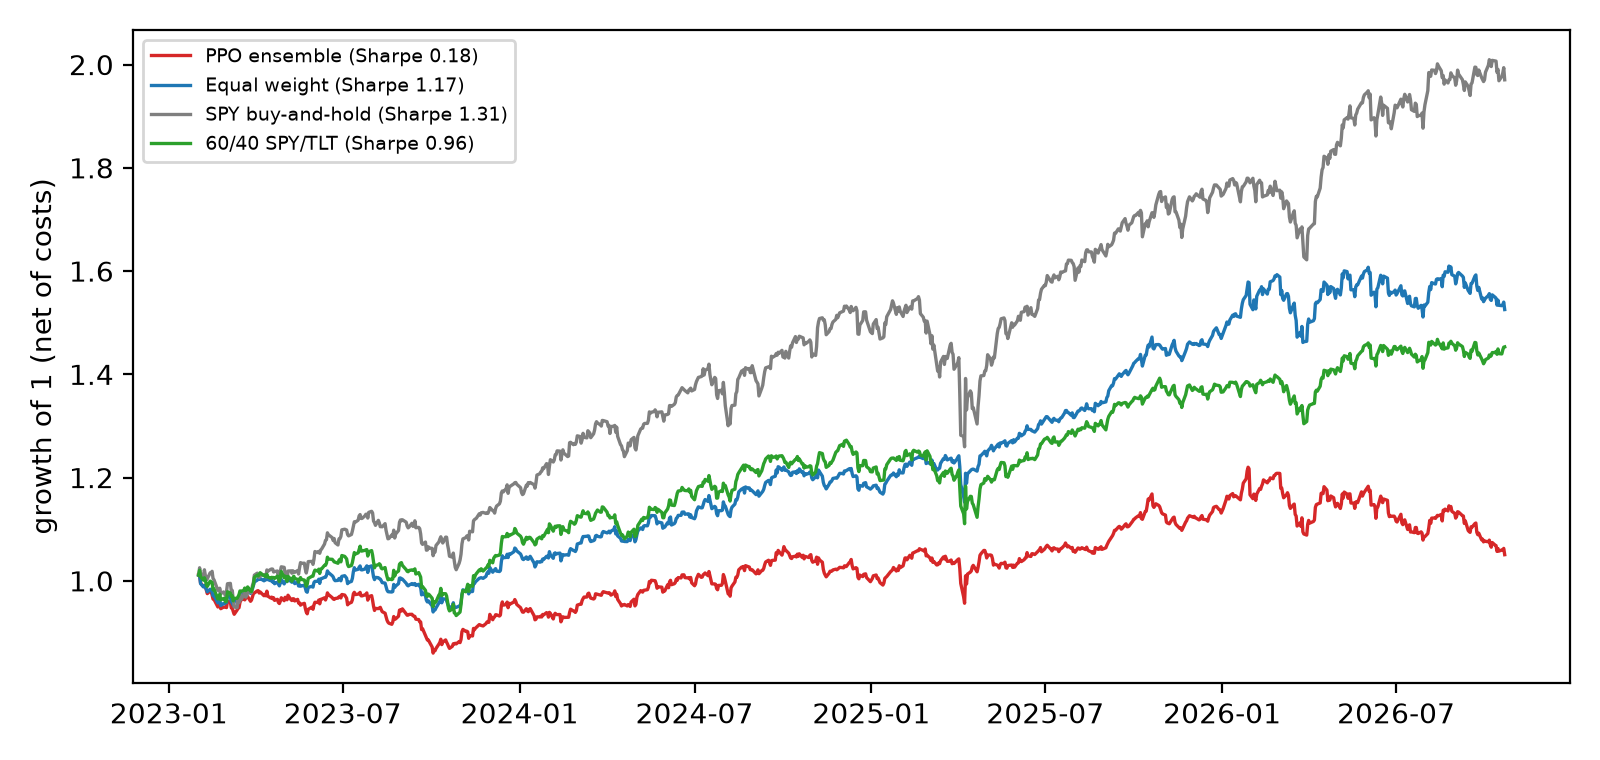
\includegraphics[width=0.85\textwidth]{fig1_rl_equity_curves.png}
\caption{Out-of-sample growth of one unit.}
\end{figure}

\section{Limitations}
Five ETFs and a single three-year test window give low statistical power; cash and financing are ignored; PPO hyper-parameters were fixed a priori, not searched, and results vary across seeds (averaged here).


\bibliographystyle{plainnat}
\bibliography{references}

\end{document}
